\begin{figure}
\centering
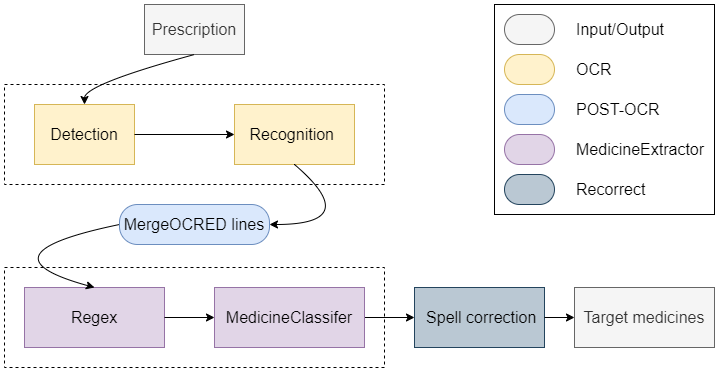
\includegraphics[width=0.7\textwidth]{method/proposed_method.png}
\caption{The architecture of Medicines Extraction on Prescription (MEP) system}\label{fig_proposed}
\end{figure}

Fig.3 exhibits the drug name recognition system MEP. It takes as input a prescription picture and feeds it into the detection model to detect the text region in the prescription. As stated, CRAFT generates a word-by-word bounding box that aids in the preservation of the precise medicine name as well as the tilt and skew of the input image, almost without affecting the recognition results. Therefore, CRAFT is well suited to the task of recognizing text in prescriptions. To recognize the detected text, the detection output is supplied into the recognition model. VietOCR is used in the text recognition stage due to its minimal complexity, high accuracy, and faster processing time than current popular models such as Tesseract. To keep the medicine's text, various vital drug names extraction methods and post-OCR procedures such as regex and MergeOCRED lines are employed. The Medicine classifier, in conjunction with the Correction approach, would provide the precise name of the medicine in the prescription.
\subsection{Craft-text-detector}
Compared to CRAFT, CTPN detects an entire row of text, which helps to maintain their coherence and faster processing time. However, CTPN does not handle tilted and skewed images effectively. Therefore, in this paper, we use the craft-text-detector, a library released by Fatih Cagatay Akyon framework to detect the text area. Based on the bounding boxes surrounding the words obtained from the conventional CRAFT architecture, this library conducts to group words on the same line/region into an object by applying thresholds. It not only creates the same effect as using CTPN but also retains the advantages of CRAFT.
\subsection{VietOCR}
VietOCR is an open-source Vietnamese text recognition model for that can be used with both handwriting and print. It was first released in 2020 by Quoc Pham and has been continuously updated in the past time. In the two Seq2Seq and Transformer installation methods, we use the former because the detection time is faster and the accuracy is not significantly different from the latter. VietOCR gets high accuracy even on a new datasets. Currently, VietOCR only supports text recognition line by line. Therefore when we have an image with many lines, we need to use supporting techniques to split the text into multiple lines first. This work we did in the craft-text-detector step. Specifically, the original image is divided into smaller images, containing the detected text areas and then inserted into VietOCR to return the resulting string.

\subsection{Medicine extractor}
% The recognition results include the whole existing text extracted from the input prescription. Aside from the name of drugs, prescriptions also contain data, such as patient information, drug dispensing facility information, disease diagnosis, and drug dosage, which are not our concerns. Therefore, there is a need to separate the drug names lines from the OCR result.  
Prescriptions, like receipts, frequently share the same qualities. The information is often provided in a systematic or semi-structured manner. Drug names are frequently listed in a consistent order and with the same pattern. By using two fundamental regular expressions, we may ease the separation of medicine names from prescriptions: 

\begin{figure}
\centering
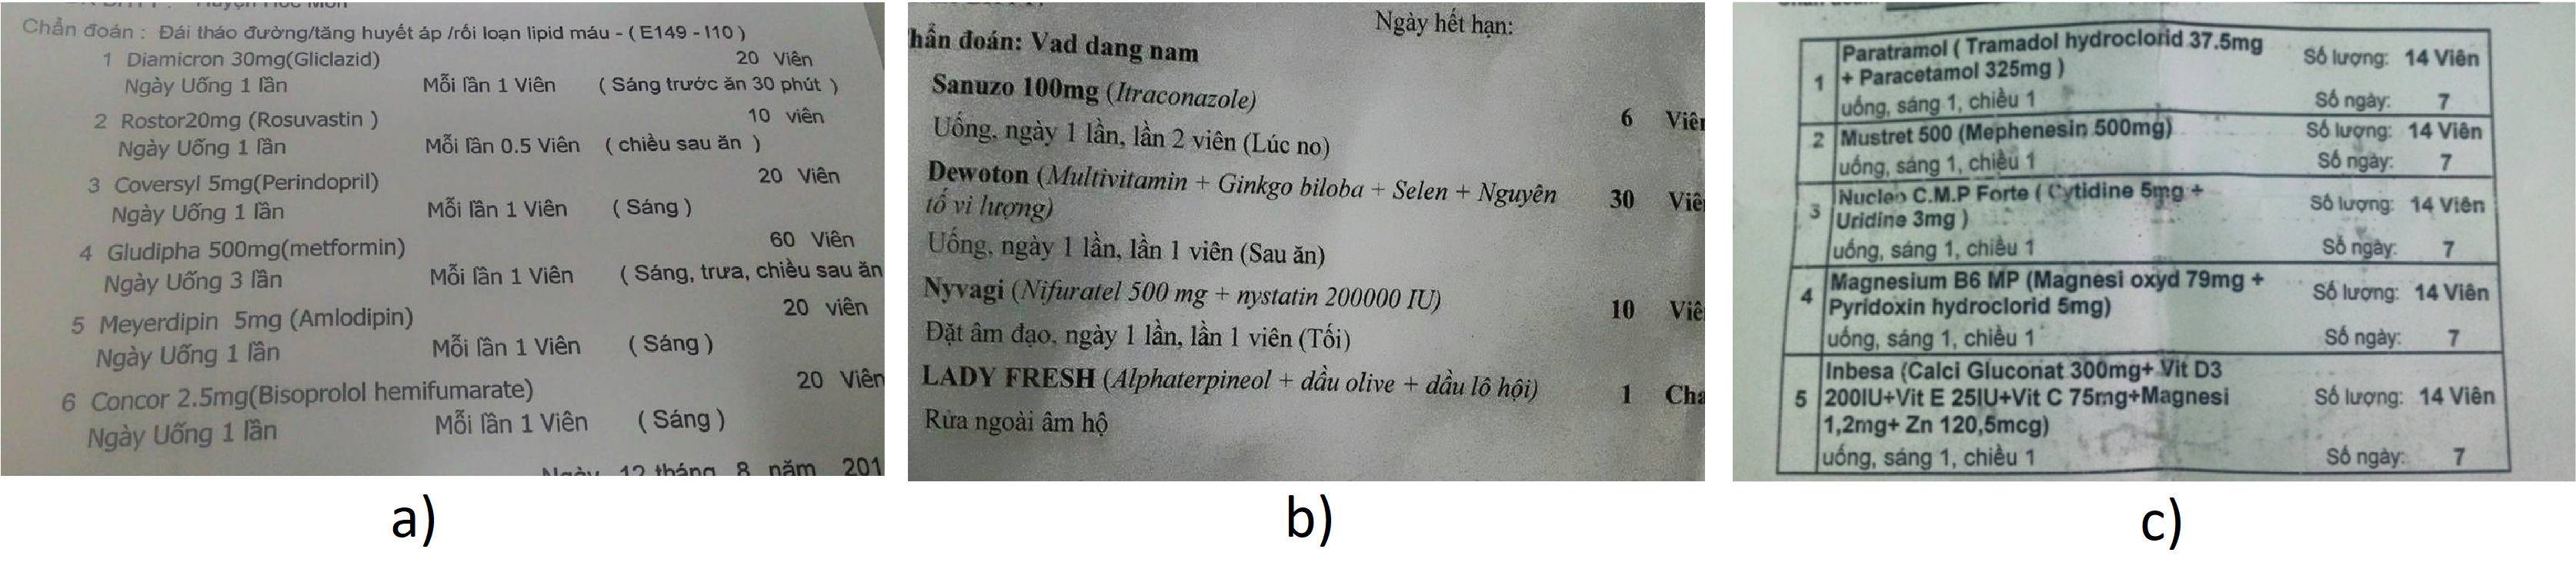
\includegraphics[width=0.8\textwidth]{method/regex_1_crop.png}
\caption{An example of prescription templates a) Medicine lines start with number, followed by medicine and ingredient b) Medicine lines start without number, followed by medicine and ingredient c) Prescription with medicine in multi-line} \label{fig_regex_1}
\end{figure}

\begin{itemize}
% \item[-] The drug names in a prescription are usually numbered. Each line starts with a number, followed by the drug name and possibly an additional active ingredient. This rule can extract the minimum of lines in the prescription and generate the highest probability of containing the drug name.

% \item[-] We modified the above rule for unnumbered prescription forms by defining the line containing the drug name that persisted according to the drug name structure followed by the active ingredient. Although this rule increases the number of lines that could be matched, it ensures the performance of the model, as well as a backup step if the OCR step cannot recognize the number before the drug name. 
\item[-] Lines containing a drug name often begin with a number, followed by a brand-name drug and possibly an active components. This rule can extract the minimum of lines in the prescription while increasing the likelihood of including the drug names.
\item[-] We extend the preceding rule for unnumbered prescription forms by specifying the line containing this structure. Although it increases the number of unrelated lines that may be matched, this technique assures the model's performance and serves as a backup step if the OCR step cannot recognize the number stand in front of the medicine name. 
\end{itemize}

Furthermore, some prescriptions include medicine names and active components spread across numerous lines. However, this is only a rare occurrence, so we do not handle it to avoid affecting the model's overall performance.
Fig.~\ref{fig_regex_1} shows examples of these format in prescription.  

After this phase, lines with a high likelihood of holding drug names would be extracted. In previous work, the entire output of the OCR matched the drug dictionary, causing the matching cost to grow as the size of the drug dictionary increased. To address this issue, the output of this step would be provided in medicine classifier Module.
\subsection{MergeOCR}
To ensure that regular expression in medicine extractor works correctly, lines containing drug names need to be bounded into boxes with all the necessary parts. However, if the image is fuzzy or noisy, the OCR process may not function properly. Rather of a single bounding box including all of digits, drug names, and drug ingredients, OCR generates numerous bounding boxes containing the separate components As a result, the extract medicine step may not work because it does not match the regular expression. Fig.~\ref{fig_merge} a) denotes a skewed text, one of the challenges of the OCR task
\begin{figure}
\centering
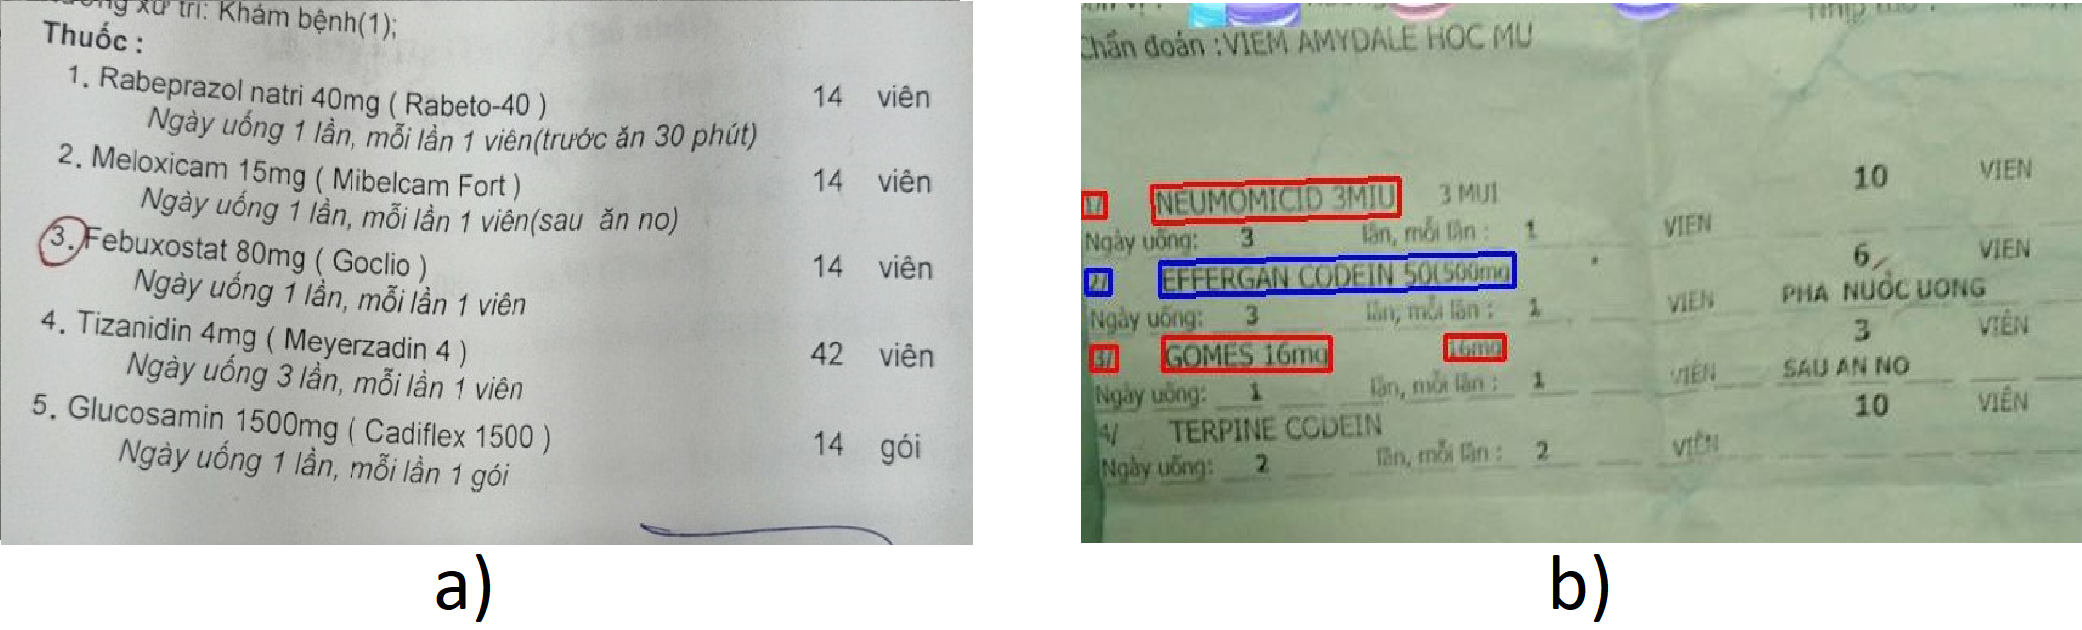
\includegraphics[width=0.9\textwidth]{method/merge_grouped.png}
\caption{a) An example show texts in prescription being skewed b) Result of MergeOCR, pieces of bounding box belong to a single line are merged correctly}
\label{fig_merge}
\end{figure}

To overcome this problem, an extended step named MergeOCR is recommended to group bounding boxes of texts belonging to the same line into a single line of text. % In addition to a line being split into different bounding boxes,  the boundaries among these bounding boxes could not be separated. Therefore, the proposed algorithm needs to overcome both these aspects effectively. Specifically, w
The AHC (Agglomerative Hierarchical Clustering) technique is used. The distance of the two bounding cells is calculated based on the y-axis coordinate distance on the 2D coordinate system. The principal advantage of AHC is that it is efficient and straightforward for this case. There is no need to predetermine the number of clusters, often referred as the number of lines in prescription. 
In this way, groups of words that are closest to each other could be prioritized and set thresholds to finish the merge process to optimize performance quickly. As merging OCR result texts is performed after the recognition step, the bounding boxes located on a line are still recognized separately, which makes VietOCR's recognition more effective and avoids interference. After the MergeOCR step, strings corresponding to the bounding box could join the correct x-axis order on the 2D coordinate system. %This line pooling makes much sense for the model before putting the data into the regex to extract the drug names. 
Fig.~\ref{fig_merge} b) shows the result of MergeOCR when grouping bounding boxes.
\subsection{Medicine Classifier}
\begin{figure}
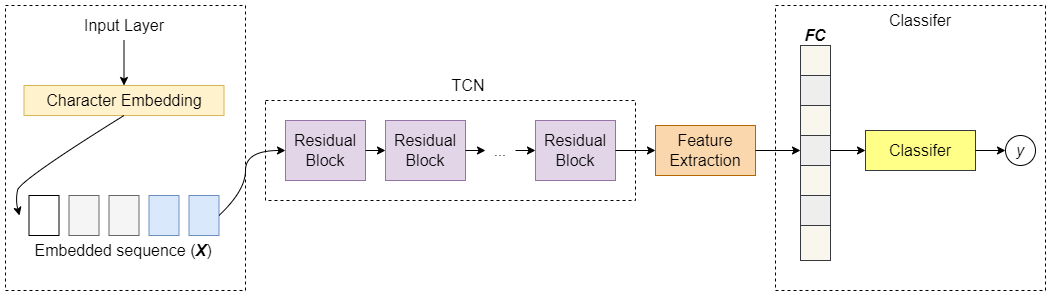
\includegraphics[width=\textwidth]{method/classifer_0.png}
\caption{Proposed medicine classifier architecture} \label{fig_class_0}
\end{figure}
After extracting lines containing drug names, the next task is to get the exact drug name in these lines. In particular, although most prescriptions have a fixed form with ordinal numbers, there is no common standard for the order between drug names and active ingredients. The drug name can precede the ingredients or vice versa, or even cases have no ingredients in that line. Therefore, the model needs to help classify a piece of text as a drug name or not, and simultaneously reduce the processing time of the entire output. %, and solve the problem more accurately. 
Based on the analyzed advantages of the TCN, it is used for this medicine classification model. Fig.~\ref{fig_class_0} shows the architecture of medicine classifier. 
The model structure includes two main parts, specifically as follows. In the first part, the input text would be pushed through the character embedding to convert to a sequence of characters. Then through padding with the longest sentence in the training phase, we represent different sentences of the same size. %Text classification is often applied to classify a whole sentence, paragraph, or essay. Therefore, people often use word embedding to help the model learn the text context better by the association among words. However,  it is short-text in medicine names. Only a few words are maximum. Drug names are often composed of several characters that are meaningless when put together, unlike the structure of ordinary words. Therefore, we propose using character embedding instead of word one. This way can both fix the problem and deal with misspelling medicine names. A long enough sequence for short-text could be obtained when using character embedding that limits overfitting. 
The second part is the TCN model, which aids to learn the features of the character embedding sequence. Because a missing or incorrect character has no effect on the overall strings, it is guaranteed to operate even if the drug names are misspelled. Furthermore, TCN's performance is extremely good. It can processing a large amount of data in a short period of time. TCN output is sent to fully connected layers, where it is classified into three categories: medicine names, active components, and others. 
% We collect data to train MedicineClassifier from drug dictionaries, which contain both medicine names and ingredients. For other classes, they are labeled as non-medicine or non-ingredient. All training data are filtered and cleaned to have the same min, max, mean and median features. Moreover, to ensure labels are in the short text, the number of words must be smaller than five
\subsection{Context-aware spell correction}
% After the MedicineClassifier step, many lines not containing the medicine names or ingredients were removed. The fewer lines are retained, the shorter the processing time is that optimizes the cost of the entire system. However, there is confusion between the drug name and the ingredient. 

\begin{figure}
\centering
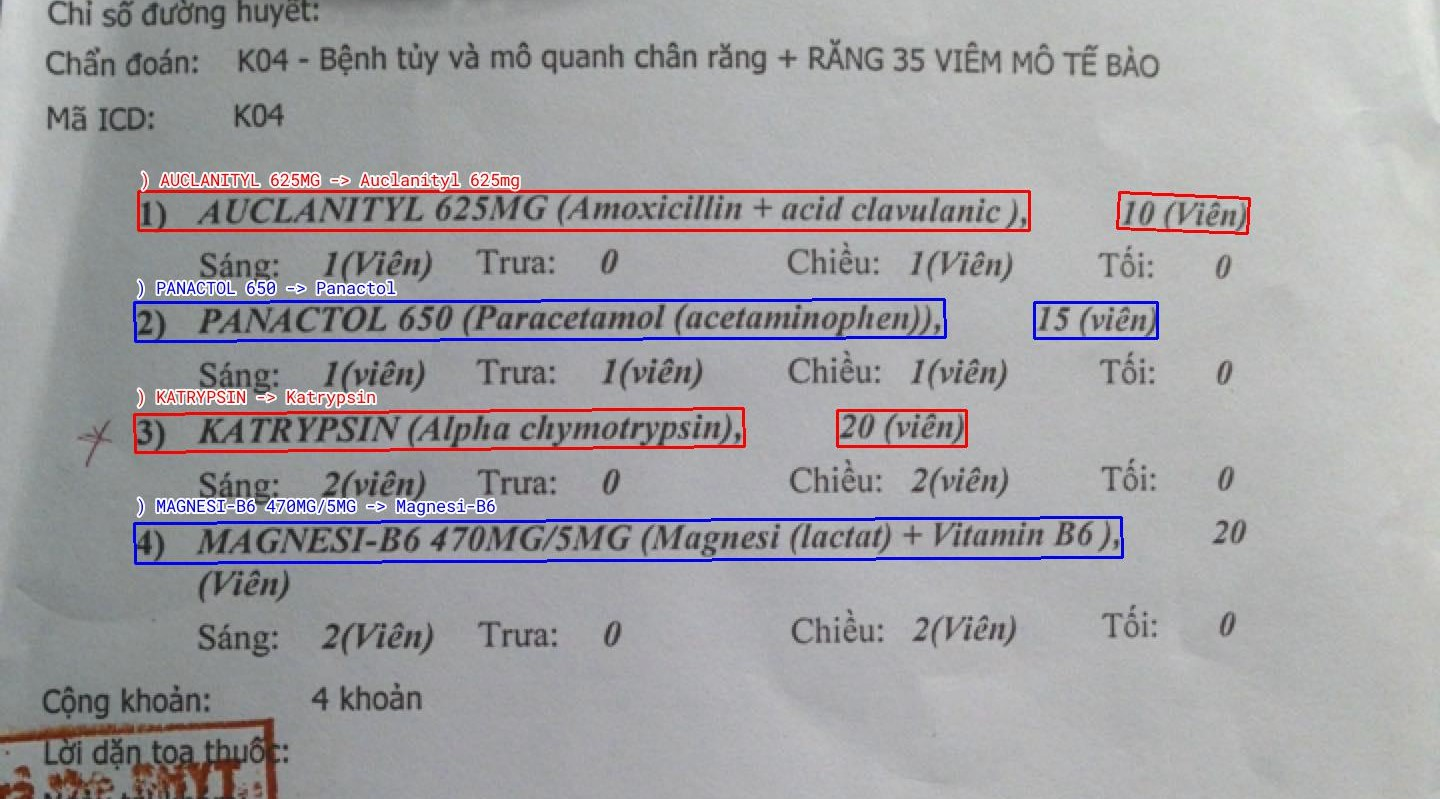
\includegraphics[width=0.7\textwidth]{method/fuzzy_0.jpg}
\caption{Corrected output of proposed Prescription Recognition system} \label{fig_fuzzy_0}
\end{figure}
A drug name sometimes could be also the ingredient and vice versa, but the medicine classifier model divided them into either drug names or ingredients. By using threshold, this last step filters the remaining lines to extract the most likely of being drug names by comparing each of them with a limited medicine names dictionary, then correcting them. This matching principle is based on edit distance, e.g. Levenshtein mentioned in previous work \cite{nguyen2021developing}, is the number of steps it takes to transform one string into another, used in many post-processing methods. 
Fig.~\ref{fig_fuzzy_0} shows our overall system's output applied spell correction.
% Sometimes, the drug name is both the ingredient and vice versa, but MedicineClassifier model divided them into either drug names or ingredients. Therefore, this last step filters the remaining lines to extract the most likely of being drug names by comparing each of them with a limited dictionary of drug names. If the match rate is higher than a threshold, it would be kept and corrected to the exact drug name in the dictionary. This matching principle is based on the edit distance, which is the number of steps it takes to transform one string into another. The smaller the number of steps, the more similar these two sequences are. Since our dictionary is a medical-specific lexicon collected from DrugBank Vietnam, the final results would be OCR error-free and only contain proper drug names. This way enhances the cost and accuracy of the system. For example, the word \emph{augmenta} has the same distance as \emph{augmentin} and \emph{augmented}. However, \emph{augmentin} would be chosen, as it is the accurate name of the medicine, while \emph{augmented} does not exist in the dictionary. 

% In previous work \cite{nguyen2021developing}, Levenshtein is mentioned as a metric for edit distance, used in many post-processing methods. The Levenshtein-based distance calculation method is leveraged to ensure the model's accuracy. However, there are some cases that both drug names and active ingredients match the dictionary. Unique drug names having the highest possibility of being medicines in the output of MedicineClassifier would be chosen. Fig.~\ref{fig_fuzzy_0} shows our overall system's output applied spell correction.

